\documentclass[12pt]{article}
\usepackage[utf8]{inputenc}
\usepackage{amssymb}
\usepackage{amsfonts}
\usepackage{color}
\usepackage{listings}
\usepackage{tikz}
\usetikzlibrary{automata,positioning,arrows}

\title{Tarea 8 \\ Programación Avanzada \\ Postgrado IIMAS }
\author{Fabián Romero}
\begin{document}
\lstset{language=bash,basicstyle=\tiny}
\maketitle

\begin{enumerate}

\item[\bf{Problema 1}]En una base de datos postgres cree una base de datos que se llame ``pavanzada'' y que pertenezca al usuario ``progavanz'', opcionalmente puede llevar la contraseña ``hola''. A continuación cree dos tablas con el archivo
adjunto pavanzada.sql desde la interfase de consola psql utilizando el comando \i (consulte la documentación).
Ahora con un proyecto roo cree una aplicación web de altas, bajas y modificaciones de las dos tablas. El proyecto roo debe de ser mandado al ayudante

\item[\bf{Postgres}]
Copiamos el archivo enviado a /tmp \\
Una vez instalado postgres y como usuario postgres se corren los siguientes comandos 
\begin{lstlisting}[frame=single] 
postgres@fabian:~$ createuser --password
Enter name of role to add: progavanz
Shall the new role be a superuser? (y/n) y
Password: (hola)

postgres@fabian:~$ psql
psql (9.1.10)
Type "help" for help.

postgres=# create database pavanzada;
CREATE DATABASE
postgres=# grant all privileges on database 
postgres=# pavanzada to progavanz;
GRANT

postgres@fabian:~$ psql pavanzada </tmp/pavanzada.sql 
SET
SET
SET
SET
SET
CREATE EXTENSION
COMMENT
SET
SET
SET
CREATE TABLE
ALTER TABLE
CREATE SEQUENCE
ALTER TABLE
ALTER SEQUENCE
CREATE TABLE
ALTER TABLE
CREATE SEQUENCE
ALTER TABLE
ALTER SEQUENCE
ALTER TABLE
ALTER TABLE
 setval 
--------
     32
(1 row)

 setval 
--------
      1
(1 row)

ALTER TABLE
ALTER TABLE
ALTER TABLE
\end{lstlisting}

Aqui tenemos creada entonces la base de datos  ``pavanzada'' que pertenece al usuario ``progavanz'' y con la contraseña ``hola''

\item[\bf{roo}]
Una vez instalada spring tool suite, creamos un directorio y corremos roo en el.
\begin{lstlisting}[frame=single] 
mkdir ~/workspace/maestria/programacion-avanzada/tarea8
cd ~/workspace/maestria/programacion-avanzada/tarea8
roo
    ____  ____  ____
   / __ \/ __ \/ __ \ 
  / /_/ / / / / / / / 
 / _, _/ /_/ / /_/ /  
/_/ |_|\____/\____/    1.2.4.RELEASE [rev 75337cf]

Welcome to Spring Roo. For assistance press TAB or type "hint" then hit ENTER.
\end{lstlisting}

Creamos el proyecto 
\begin{lstlisting}[frame=single] 
roo> project --topLevelPackage mx.unam.mcc.pa --projectName problema1
Created ROOT/pom.xml
Created SRC_MAIN_RESOURCES
Created SRC_MAIN_RESOURCES/log4j.properties
Created SPRING_CONFIG_ROOT
Created SPRING_CONFIG_ROOT/applicationContext.xml
\end{lstlisting}

Establecemos el uso de datos

\begin{lstlisting}[frame=single] 
roo> persistence setup --database POSTGRES --provider OPENJPA
Created SPRING_CONFIG_ROOT/database.properties
Please update your database details in 
src/main/resources/META-INF/spring/database.properties.
\end{lstlisting}

En este momento nos solicita establecer correctamente el archivo database.properties que lo establecemos así:

\begin{lstlisting}[frame=single] 
database.driverClassName=org.postgresql.Driver
database.url=jdbc\:postgresql\://localhost\:5432/pavanzada
database.username=progavanz
database.password=hola
\end{lstlisting}

Probamos la conexión. Pero como no tiene todavia los drivers de Postgres nos pide instalarlos
\begin{lstlisting}[frame=single] 
roo> database introspect --schema public
Located add-ons that may offer this JDBC driver
2 found, sorted by rank; T = trusted developer; R = Roo 1.2 compatible
ID T R DESCRIPTION -------------------------------------------------------------
01 Y Y 9.1.0.901-1_0001 Postgres #jdbcdriver...
02 Y Y 9.1.0.901_0001 Postgres #jdbcdriver...
--------------------------------------------------------------------------------
JDBC driver not available for 'org.postgresql.Driver'
roo> addon install bundle --bundleSymbolicName 
addon install bundle --bundleSymbolicName 
required --bundleSymbolicName: The bundle symbolic name for the add-on of interest; 
no default value
\end{lstlisting}

Lo instalamos tal como lo sugiere:
\begin{lstlisting}[frame=single] 
roo> addon install id --searchResultId 01
Target resource(s):
-------------------
   Spring Roo - Wrapping - postgresql-jdbc4 (9.1.0.901-1_0001)

Deploying...done.

Successfully installed add-on: Spring Roo - Wrapping - postgresql-jdbc4 
[version: 9.1.0.901-1_0001]
\end{lstlisting}

Y probamos de nuevo la conexión
\begin{lstlisting}[frame=single] 
roo> database introspect --schema public
<?xml version="1.0" encoding="UTF-8" standalone="no"?>
<!--WARNING: DO NOT EDIT THIS FILE. THIS FILE IS MANAGED BY SPRING ROO.-->
<database name="deprecated">
    <option key="moduleName" value=""/>
    <option key="activeRecord" value="false"/>
    <option key="repository" value="false"/>
    <option key="service" value="false"/>
    <option key="includeNonPortableAttributes" value="true"/>
    <option key="disableVersionFields" value="true"/>
    <option key="disableGeneratedIdentifiers" value="true"/>
    <option key="testAutomatically" value="false"/>
    <table alias="public" name="estado">
        <column name="id" primaryKey="true" required="true" scale="0" 
                size="10" type="4,serial"/>
        <column name="pais" primaryKey="false" required="false" scale="0" 
                size="100" type="12,varchar"/>
        <column name="estado" primaryKey="false" required="false" scale="0" 
                size="100" type="12,varchar"/>
        <foreign-key foreignTable="usuario" name="usuario_id_est_fkey" 
                onDelete="none" onUpdate="none">
            <option key="foreignSchemaName" value="public"/>
            <option key="exported" value="true"/>
            <reference foreign="id_est" local="id"/>
        </foreign-key>
        <unique name="estado_pkey">
            <unique-column name="id"/>
        </unique>
    </table>
    <table alias="public" name="usuario">
        <column name="id" primaryKey="true" required="true" scale="0" 
                size="10" type="4,serial"/>
        <column name="nombre" primaryKey="false" required="false" 
                scale="0" size="100" type="12,varchar"/>
        <column name="apellidos" primaryKey="false" required="false" 
                scale="0" size="200" type="12,varchar"/>
        <column name="id_est" primaryKey="false" required="false" 
                scale="0" size="10" type="4,int4"/>
        <foreign-key foreignTable="estado" name="usuario_id_est_fkey" 
                onDelete="none" onUpdate="none">
            <option key="foreignSchemaName" value="public"/>
            <option key="exported" value="false"/>
            <reference foreign="id" local="id_est"/>
        </foreign-key>
        <unique name="usuario_pkey">
            <unique-column name="id"/>
        </unique>
    </table>
</database>
\end{lstlisting}

Como ya esta conectando correctamente, procedemos a crear el modelo en base a la estructura de la base de datos

\begin{lstlisting}[frame=single] 
roo> database reverse engineer --schema public
Created SRC_MAIN_RESOURCES/dbre.xml
Updated ROOT/pom.xml
Updated SRC_MAIN_RESOURCES/META-INF/persistence.xml
Created SRC_MAIN_JAVA/mx/unam/mcc/pa
Created SRC_MAIN_JAVA/mx/unam/mcc/pa/Estado.java
Created SRC_MAIN_JAVA/mx/unam/mcc/pa/Usuario.java
Updated SRC_MAIN_JAVA/mx/unam/mcc/pa/Estado.java
Updated SRC_MAIN_JAVA/mx/unam/mcc/pa/Usuario.java
Created SRC_MAIN_JAVA/mx/unam/mcc/pa/Estado_Roo_Configurable.aj
Created SRC_MAIN_JAVA/mx/unam/mcc/pa/Estado_Roo_Jpa_ActiveRecord.aj
Created SRC_MAIN_JAVA/mx/unam/mcc/pa/Estado_Roo_DbManaged.aj
Created SRC_MAIN_JAVA/mx/unam/mcc/pa/Estado_Roo_ToString.aj
Created SRC_MAIN_JAVA/mx/unam/mcc/pa/Estado_Roo_Jpa_Entity.aj
Created SRC_MAIN_JAVA/mx/unam/mcc/pa/Usuario_Roo_Configurable.aj
Created SRC_MAIN_JAVA/mx/unam/mcc/pa/Usuario_Roo_Jpa_ActiveRecord.aj
Created SRC_MAIN_JAVA/mx/unam/mcc/pa/Usuario_Roo_DbManaged.aj
Created SRC_MAIN_JAVA/mx/unam/mcc/pa/Usuario_Roo_ToString.aj
Created SRC_MAIN_JAVA/mx/unam/mcc/pa/Usuario_Roo_Jpa_Entity.aj
\end{lstlisting}

Inicializamos una  aplicación web.

\begin{lstlisting}[frame=single] 
roo> web mvc setup
Created ROOT/src/main/webapp/WEB-INF/spring
Created ROOT/src/main/webapp/WEB-INF/spring/webmvc-config.xml
Created ROOT/src/main/webapp/WEB-INF/web.xml
Updated ROOT/src/main/webapp/WEB-INF/spring/webmvc-config.xml
Created ROOT/src/main/webapp/images
Created ROOT/src/main/webapp/images/add.png
Created ROOT/src/main/webapp/images/banner-graphic.png
Created ROOT/src/main/webapp/images/create.png
Created ROOT/src/main/webapp/images/delete.png
Created ROOT/src/main/webapp/images/favicon.ico
Created ROOT/src/main/webapp/images/list.png
Created ROOT/src/main/webapp/images/resultset_first.png
Created ROOT/src/main/webapp/images/resultset_last.png
Created ROOT/src/main/webapp/images/resultset_next.png
Created ROOT/src/main/webapp/images/resultset_previous.png
Created ROOT/src/main/webapp/images/show.png
Created ROOT/src/main/webapp/images/springsource-logo.png
Created ROOT/src/main/webapp/images/update.png
Created ROOT/src/main/webapp/styles
Created ROOT/src/main/webapp/styles/alt.css
Created ROOT/src/main/webapp/styles/standard.css
Created ROOT/src/main/webapp/WEB-INF/classes
Created ROOT/src/main/webapp/WEB-INF/classes/alt.properties
Created ROOT/src/main/webapp/WEB-INF/classes/standard.properties
Created ROOT/src/main/webapp/WEB-INF/layouts
Created ROOT/src/main/webapp/WEB-INF/layouts/default.jspx
Created ROOT/src/main/webapp/WEB-INF/layouts/layouts.xml
Created ROOT/src/main/webapp/WEB-INF/views
Created ROOT/src/main/webapp/WEB-INF/views/header.jspx
Created ROOT/src/main/webapp/WEB-INF/views/menu.jspx
Created ROOT/src/main/webapp/WEB-INF/views/footer.jspx
Created ROOT/src/main/webapp/WEB-INF/views/views.xml
Created ROOT/src/main/webapp/WEB-INF/views/dataAccessFailure.jspx
Created ROOT/src/main/webapp/WEB-INF/views/index-template.jspx
Created ROOT/src/main/webapp/WEB-INF/views/index.jspx
Created ROOT/src/main/webapp/WEB-INF/views/resourceNotFound.jspx
Created ROOT/src/main/webapp/WEB-INF/views/uncaughtException.jspx
Created ROOT/src/main/webapp/WEB-INF/tags/form
Created ROOT/src/main/webapp/WEB-INF/tags/form/create.tagx
Created ROOT/src/main/webapp/WEB-INF/tags/form/dependency.tagx
Created ROOT/src/main/webapp/WEB-INF/tags/form/find.tagx
Created ROOT/src/main/webapp/WEB-INF/tags/form/list.tagx
Created ROOT/src/main/webapp/WEB-INF/tags/form/show.tagx
Created ROOT/src/main/webapp/WEB-INF/tags/form/update.tagx
Created ROOT/src/main/webapp/WEB-INF/tags/form/fields
Created ROOT/src/main/webapp/WEB-INF/tags/form/fields/checkbox.tagx
Created ROOT/src/main/webapp/WEB-INF/tags/form/fields/column.tagx
Created ROOT/src/main/webapp/WEB-INF/tags/form/fields/datetime.tagx
Created ROOT/src/main/webapp/WEB-INF/tags/form/fields/display.tagx
Created ROOT/src/main/webapp/WEB-INF/tags/form/fields/editor.tagx
Created ROOT/src/main/webapp/WEB-INF/tags/form/fields/input.tagx
Created ROOT/src/main/webapp/WEB-INF/tags/form/fields/reference.tagx
Created ROOT/src/main/webapp/WEB-INF/tags/form/fields/select.tagx
Created ROOT/src/main/webapp/WEB-INF/tags/form/fields/simple.tagx
Created ROOT/src/main/webapp/WEB-INF/tags/form/fields/table.tagx
Created ROOT/src/main/webapp/WEB-INF/tags/form/fields/textarea.tagx
Created ROOT/src/main/webapp/WEB-INF/tags/menu
Created ROOT/src/main/webapp/WEB-INF/tags/menu/category.tagx
Created ROOT/src/main/webapp/WEB-INF/tags/menu/item.tagx
Created ROOT/src/main/webapp/WEB-INF/tags/menu/menu.tagx
Created ROOT/src/main/webapp/WEB-INF/tags/util
Created ROOT/src/main/webapp/WEB-INF/tags/util/language.tagx
Created ROOT/src/main/webapp/WEB-INF/tags/util/load-scripts.tagx
Created ROOT/src/main/webapp/WEB-INF/tags/util/pagination.tagx
Created ROOT/src/main/webapp/WEB-INF/tags/util/panel.tagx
Created ROOT/src/main/webapp/WEB-INF/tags/util/placeholder.tagx
Created ROOT/src/main/webapp/WEB-INF/tags/util/theme.tagx
Created ROOT/src/main/webapp/WEB-INF/i18n
Created ROOT/src/main/webapp/WEB-INF/i18n/messages.properties
Created ROOT/src/main/webapp/images/en.png
Updated ROOT/src/main/webapp/WEB-INF/i18n/application.properties
Updated ROOT/src/main/webapp/WEB-INF/web.xml
Updated ROOT/pom.xml [added dependencies ...]
Updated SRC_MAIN_WEBAPP/WEB-INF/views/footer.jspx
\end{lstlisting}

Agregamos también el Scaffolding correspondiente al modelo que creamos.

\begin{lstlisting}[frame=single] 
roo> web mvc all --package ~.web
Created SRC_MAIN_JAVA/mx/unam/mcc/pa/web
Created SRC_MAIN_JAVA/mx/unam/mcc/pa/web/UsuarioController.java
Created SRC_MAIN_JAVA/mx/unam/mcc/pa/web/EstadoController.java
Updated SRC_MAIN_WEBAPP/WEB-INF/spring/webmvc-config.xml
Created SRC_MAIN_WEBAPP/WEB-INF/views/estadoes
Created SRC_MAIN_WEBAPP/WEB-INF/views/estadoes/views.xml
Updated SRC_MAIN_WEBAPP/WEB-INF/views/estadoes/views.xml
Updated SRC_MAIN_WEBAPP/WEB-INF/i18n/application.properties
Created SRC_MAIN_WEBAPP/WEB-INF/views/usuarios
Created SRC_MAIN_WEBAPP/WEB-INF/views/usuarios/views.xml
Updated SRC_MAIN_WEBAPP/WEB-INF/views/usuarios/views.xml
Updated SRC_MAIN_WEBAPP/WEB-INF/i18n/application.properties
Created SRC_MAIN_JAVA/mx/unam/mcc/pa/web/EstadoController_Roo_Controller.aj
Created SRC_MAIN_WEBAPP/WEB-INF/views/estadoes/list.jspx
Created SRC_MAIN_WEBAPP/WEB-INF/views/estadoes/show.jspx
Created SRC_MAIN_WEBAPP/WEB-INF/views/estadoes/create.jspx
Updated SRC_MAIN_WEBAPP/WEB-INF/views/menu.jspx
Created SRC_MAIN_WEBAPP/WEB-INF/views/estadoes/update.jspx
Created SRC_MAIN_JAVA/mx/unam/mcc/pa/web/UsuarioController_Roo_Controller.aj
Created SRC_MAIN_WEBAPP/WEB-INF/views/usuarios/list.jspx
Created SRC_MAIN_WEBAPP/WEB-INF/views/usuarios/show.jspx
Created SRC_MAIN_WEBAPP/WEB-INF/views/usuarios/create.jspx
Created SRC_MAIN_WEBAPP/WEB-INF/views/usuarios/update.jspx
\end{lstlisting}

Corremos las pruebas
\begin{lstlisting}[frame=single] 
roo> perform tests
[INFO] --- aspectj-maven-plugin:1.4:compile (default) @ problema1 ---
[INFO] No modifications found skipping aspectJ compile
[INFO] 
[INFO] --- aspectj-maven-plugin:1.4:test-compile (default) @ problema1 ---
[WARNING] No sources found skipping aspectJ compile
[INFO] 
[INFO] --- maven-resources-plugin:2.6:resources (default-resources) @ problema1 ---
[INFO] Using 'UTF-8' encoding to copy filtered resources.
[INFO] Copying 5 resources
[INFO] 
[INFO] --- maven-compiler-plugin:2.5.1:compile (default-compile) @ problema1 ---
[INFO] Nothing to compile - all classes are up to date
[INFO] 
[INFO] --- openjpa-maven-plugin:2.2.2:enhance (enhancer) @ problema1 ---
[INFO] 
[INFO] --- maven-resources-plugin:2.6:testResources @ problema1 ---
[INFO] Using 'UTF-8' encoding to copy filtered resources.
[INFO] skip non existing resourceDirectory 
/home/fabian/workspace/maestria/programacion-avanzada/tarea8/src/test/resources
[INFO] 
[INFO] --- maven-compiler-plugin:2.5.1:testCompile @ problema1 ---
[INFO] No sources to compile
[INFO] 
[INFO] --- maven-surefire-plugin:2.12:test (default-test) @ problema1 ---
[INFO] No tests to run.
[INFO] Surefire report directory: 
/home/fabian/workspace/maestria/programacion-avanzada/tarea8/target/surefire-reports
roo> 
-------------------------------------------------------
 T E S T S
-------------------------------------------------------
roo> 
Results :
roo> 
Tests run: 0, Failures: 0, Errors: 0, Skipped: 0
roo> 
[INFO] ------------------------------------------------------------------------
[INFO] BUILD SUCCESS
[INFO] ------------------------------------------------------------------------
[INFO] Total time: 2.508s
[INFO] Finished at: Sat Nov 23 22:31:29 CST 2013
[INFO] Final Memory: 14M/304M
[INFO] ------------------------------------------------------------------------
\end{lstlisting}

Salimos de roo y probamos la aplicación:

\begin{lstlisting}[frame=single] 
fabian@fabian-HP:~/workspace/maestria/programacion-avanzada/tarea8$ mvn jetty:run
[INFO] Scanning for projects...
[INFO]                                                                         
[INFO] ------------------------------------------------------------------------
[INFO] Building problema1 0.1.0.BUILD-SNAPSHOT
[INFO] ------------------------------------------------------------------------
[INFO] 
[INFO] >>> jetty-maven-plugin:8.1.4.v20120524:run (default-cli) @ problema1 >>>
[INFO] 
[INFO] --- aspectj-maven-plugin:1.4:compile (default) @ problema1 ---
[INFO] No modifications found skipping aspectJ compile
[INFO] 
[INFO] --- aspectj-maven-plugin:1.4:test-compile (default) @ problema1 ---
[WARNING] No sources found skipping aspectJ compile
[INFO] 
[INFO] --- maven-resources-plugin:2.6:resources (default-resources) @ problema1 ---
[INFO] Using 'UTF-8' encoding to copy filtered resources.
[INFO] Copying 5 resources
[INFO] 
[INFO] --- maven-compiler-plugin:2.5.1:compile (default-compile) @ problema1 ---
[INFO] Nothing to compile - all classes are up to date
[INFO] 
[INFO] --- openjpa-maven-plugin:2.2.2:enhance (enhancer) @ problema1 ---
[INFO] 
[INFO] --- maven-resources-plugin:2.6:testResources  @ problema1 ---
[INFO] 
[INFO] --- maven-compiler-plugin:2.5.1:testCompile   @ problema1 ---
[INFO] No sources to compile
[INFO] 
[INFO] <<< jetty-maven-plugin:8.1.4.v20120524:run (default-cli) @ problema1 <<<
[INFO] 
[INFO] --- jetty-maven-plugin:8.1.4.v20120524:run (default-cli) @ problema1 ---
[INFO] Configuring Jetty for project: problema1
[INFO] Reload Mechanic: automatic
[INFO] Classes = /home/fabian/workspace/maestria/programacion-avanzada/tarea8/
target/classes
[INFO] Context path = /problema1
[INFO] Tmp directory = /home/fabian/workspace/maestria/programacion-avanzada/
tarea8/target/tmp
[INFO] Web defaults = org/eclipse/jetty/webapp/webdefault.xml
[INFO] Web overrides =  none
[INFO] web.xml file = file:/home/fabian/workspace/maestria/programacion-avanzada/
tarea8/src/main/webapp/WEB-INF/web.xml
[INFO] Webapp directory = /home/fabian/workspace/maestria/programacion-avanzada/
tarea8/src/main/webapp
2013-11-23 22:31:48.120:INFO:oejs.Server:jetty-8.1.4.v20120524
2013-11-23 22:31:48.960:INFO:oejpw.PlusConfiguration:No Transaction manager found 
- if your webapp requires one, please configure one.
2013-11-23 22:31:50.760:INFO:/problema1:No Spring WebApplicationInitializer 
types detected on classpath
2013-11-23 22:31:51:INFO:oejsh.ContextHandler:started o.m.j.p.JettyWebAppContext
{/problema1,file:/home/fabian/workspace/maestria/programacion-avanzada/tarea8/src/
main/webapp/},file:/home/fabian/workspace/maestria/programacion-avanzada/tarea8/
src/main/webapp/
2013-11-23 22:31:51:INFO:oejsh.ContextHandler:started o.m.j.p.JettyWebAppContext
{/problema1,file:/home/fabian/workspace/maestria/programacion-avanzada/tarea8/src/
main/webapp/},file:/home/fabian/workspace/maestria/programacion-avanzada/tarea8/
/main/webapp/
2013-11-23 22:31:51:INFO:oejsh.ContextHandler:started o.m.j.p.JettyWebAppContext
{/problema1,file:/home/fabian/workspace/maestria/programacion-avanzada/tarea8/src
/main/webapp/},file:/home/fabian/workspace/maestria/programacion-avanzada/tarea8/
/main/webapp/
2013-11-23 22:31:51:INFO:/problema1:Initializing Spring root WebApplicationContext
2013-11-23 22:31:51:INFO:oejsh.ContextHandler:started o.m.j.p.JettyWebAppContext
{/problema1,file:/home/fabian/workspace/maestria/programacion-avanzada/tarea8/
main/webapp/},file:/home/fabian/workspace/maestria/programacion-avanzada/tarea8/
src/main/webapp/
2013-11-23 22:31:51.738:INFO:/problema1:Initializing Spring FrameworkServlet 
'problema1'
2013-11-23 22:31:52.474:INFO:oejs.AbstractConnector:
Started SelectChannelConnector@0.0.0.0:8080
[INFO] Started Jetty Server
\end{lstlisting}

voilà\\
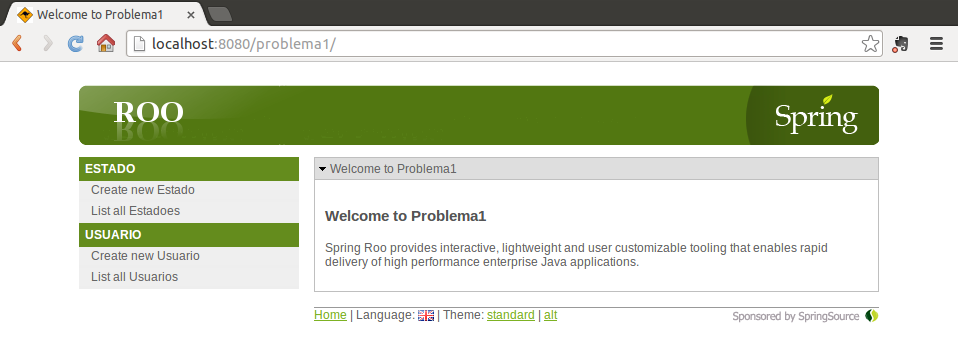
\includegraphics[width=12cm]{Screen.png}

\end{enumerate}
\end{document}
